%\documentclass[preprint]{aastex}  % USE THIS TO MAKE BIB, THEN FORMAT USING EMULATEAPJ
\documentclass[twocolumn,numberedappendix]{emulateapj}
\shorttitle{PSA64}
\shortauthors{Ali, et al.}

\usepackage{amsmath}
\usepackage{graphicx}
\usepackage[figuresright]{rotating}
%\usepackage{rotating}
\usepackage{natbib}
%\usepackage{pdflscape}
%\usepackage{lscape}
\citestyle{aa}

\def\b{\mathbf{b}}
\def\k{\mathbf{k}}
\def\r{\mathbf{r}}
\def\q{\mathbf{q}}
\def\b{\mathbf{b}}
\def\kp{\mathbf{k}^\prime}
\def\kpp{\mathbf{k}^{\prime\prime}}
\def\V{\mathbb{V}}
\def\At{\tilde{A}}
\def\Vt{\tilde{V}}
\def\Tt{\tilde{T}}
\def\tb{\langle T_b\rangle}
\newcommand{\vis}{\mathbf{v}}
\newcommand{\x}{\mathbf{x}}
\newcommand{\xhat}{\hat{\mathbf{x}}}
\newcommand{\A}{\mathbf{A}}
\newcommand{\N}{\mathbf{N}}
\newcommand{\rhat}{\hat{\mathbf{r}}}

\begin{document}
\title{PSA-64 Power Spectrum}

\author{
Zaki S. Ali\altaffilmark{1},
Aaron R. Parsons\altaffilmark{1,2},
Adrian Liu\altaffilmark{1},
Jeff Zheng
James E. Aguirre\altaffilmark{3},
David R. DeBoer\altaffilmark{2},
Daniel C. Jacobs\altaffilmark{8},
David F. Moore\altaffilmark{3},
Jonathan C. Pober\altaffilmark{4},
% XXX if includes paper data, needs full author list
}

\altaffiltext{1}{Astronomy Dept., U. California, Berkeley, CA}
\altaffiltext{2}{Radio Astronomy Lab., U. California, Berkeley, CA}
\altaffiltext{3}{Dept. of Physics and Astronomy, U. Pennsylvania, Philadelphia, PA}
\altaffiltext{4}{Physics Dept.  U. Washington, Seattle, WA}
\altaffiltext{8}{School of Earth and Space Exploration, Arizona State U., Tempe, AZ}

\begin{abstract}
\end{abstract}

% XXX fringe weighting profile
% XXX delay spectrum not violated by freq-dependent fringe rate weights

\section{Introduction}
The Donald C. Backer Precision Array for Probing the Epoch of Reionization
(PAPER) is a dedicated experiment to measure the power spectrum of highly
redshifted 21 cm emission during the Epoch of Reionization. PAPER is but one
experiment that aims to detect this faint signal. Other telescopes that have the
same goal are the Giant Meter-wave Radio Telescope (GMRT), the LOw Frequency
ARray (LOFAR), and the Murchison Widefield Array (MWA). PAPER currently consists
of 128 dual-polarization antennae in a 100-200MHz band out in the Karoo desert
in South Africa. 

The current best upper limit on 21 cm signal level is at $(41 mK)^{2}$ which was
measured by PAPER. This limit was acheived by using the delay-spectrum technique
to remove foregrounds and by using a maximum redundancy array to essentially
measure the same $k$-modes repeatedly, boosting sensitivity. In this analysis we
employ the same techniques mentioned as well is introduce an optimal fringe-fringe
rate filter to  boost sensitivity and make use of precise calibration via
the Omnical redundant calibrator package. 

The paper is outlined as follows. In section \ref{sec:observations} we describe
the observations used in this analysis. In \ref{sec:improvements} we discuss the
improvements in this pipeline with respect to the previous analysis of PSA-32
\cite{parsons_et_al2014}. We then move on to the data analysis pipeline in
section \ref{sec:analysis}. Seciton \ref{sec:results} describes the results of
 our efforts and provides new contraints on EoR. We conclude in
\ref{sec:conclusion}.


\section{Observations}\ref{sec:observations}
Here, we describe the features of the data set used in this analysis. 
Currently, PAPER boasts a modest 128 dual-polarization antenna array, which was
followed by a 64 antenna array. This paper focuses on the latter.
We used a maximally redundant configuration of the PAPER array (see Figure
\ref{fig:antenna_positions} for this analysis, relying on all of the redundant
baselines for the calibration procedure, but only using a subset of the
baselines for the power spectrum analysis. The columns are separated by 30
meters and the rows by 5 meters. For the power spectrum analysis we
are using the baselines that correspond to the width between two columns (e.g.
49-41) as well as those that correspond to over and up and down one antenna
(e.g. 10-41 and 10-58, respectively). These 154 baselines are 
instantaneously redundant and therefore they measure the same Fourier modes on
the sky. Within a single group of the three types of baselines above, the
measurements add coherently, where between groups they add in quadrature. Having
repeated measurements of the same baseline type greatly increases sensitivity. 

The observation of this 64 antenna data set spanned a 135 day period that
commenced on 2012 November 8 (JD62456240) and ended  2013 March 23 (JD62456375). 
Each baseline instantaneously measured the 100-200 MHz band which was divided
into 1024 frequency channels of resolution 97.66 kHz and integrated for 10.7
seconds. In this analysis we analyze observations that spanned, in local
siderial time (LST), a range of 1:00 to 10:00 hours. This range corresponds to
the "EoR cold patch", in which galaxtic synchrotron power is minimal (away from
the center of the galaxy).
%XXX lst range will change.

\begin{figure*}[!t]\centering
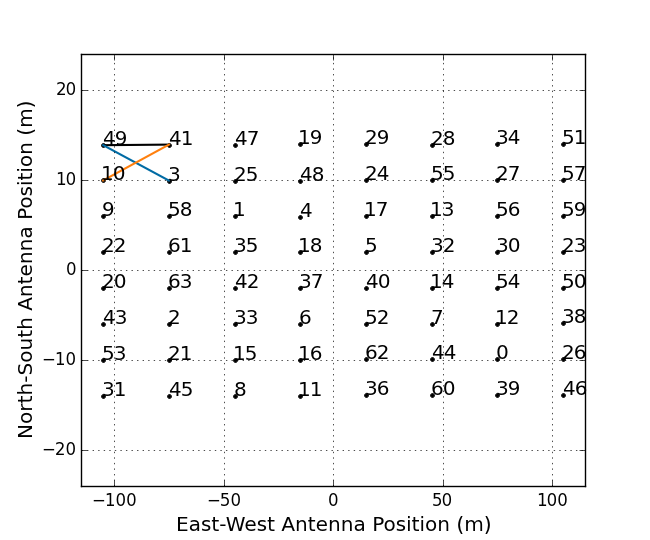
\includegraphics[width=1.85\columnwidth,height=\columnwidth]{plots/antenna_positions.png}
\caption{Antenna positions for the PAPER 64 observation run.}
\label{fig:antenna_positions}
\end{figure*}

\section{Summary of Improvements from PSA32}
In comparison to the previous PAPER pipeline (see \cite{parsons_et_al2014}),
this analysis took a slightly different approach which included some important
steps to improve our bottom line. In short, the improvements included using a
new, refined redundant calibration method (Zheng 2014), increasing the width of
the wideband delay filter that removes smothe spectrum foregrounds, weighting
the lst binned data sets, and optimal fringe rate filtering. In section
\ref{sec:analysis}, we dicuss each of the improvements in more detail.

Figure \ref{fig:step_through_pspec} (TBD) shows the power spectra when each of
the steps mentioned above are turned off and for the one where all of them are
turned on. We can see the gradual improvement of the power spectra (hopefully).


%A more rigorous calibrations. Forward Ref.
%omnical
%lstbinning with chi-sq weighting
%horizon cut at 200ns = 100 + 100 (instead of 100 + 15)
%optimal fringe-rate filtereing
%want the 4(5?) figures in this section. Incrementally step back through improvement points.


\section{Analysis}
Describe the overall flow of the data through of the pipeline.
Here we describe the analysis pipeline of the data set obtained in 2012/2013
observing season. 
Data was first run through a preprocessing compression pipeline which reduces
the volume of the data by a factor of forty. Afterwards we calibrate the
relative phases of our array on the basis of redundancy using a logcal approach
in delay space, and then get the absoultue phase calibration by fitting. We then
set the flux scale of our observations by using Pictor A. The logcal done above
was a rough estimate of the phase calibration and hence we used Omnical to get
the calibrations to higher accuracy. This was a major difference in the pipeline
from previous iterations on PAPER data. We then remove foregrounds using the
delay filtering technique and form power spectra. The detalis of the above are
discussed below and figure \ref{fig:analysis_pipeline} shows a block diagram of
the analysis pipeline.

\subsection{Preprocessing Compression}
As low frequency interferometer grow bigger, data volume becomes an issue. For
this data set a 10 minute file consisting of 1024 channel complex visibilites
integrated for 10.7 seconds each, requires 4G of storage space. For the
observing season this requires about 40TB of storage space. This is doable, for
now, but when it comes to analyzing sorting through this much data can be
cumbersome. Therfore we have implementd a compression techinque which reduces
the amount of storage by a factor of forty. 
Details of this critical step are presetned in the appendix A of
\citep{parsons2014a}.  The punch line is that after RFI flagging, and removing
unsmooth and transient emission from the data, we end up with a factor of 20
reduction in data volume, ending up with a total data set that requres 2TB of
storage. After compression, it ends up that the orignal 1024 channels get
downsampled to 203 channels (still encompassing the 100 MHz) and the 60 time
samples per 10 minute file end up as 14 timesamples with an effective
integration time of 42.8 seconds. 

(Show plot of rraw data and compressed data? )
\subsection{Calibrations}
\subsubsection{Overview}
Precise calibration turned out to be critical in improving our bottom line of
our final result. We began the calibration procedure by first using a
logarithmic calibration scheme based in redundant measurements
(\citep{liu_et_al2010}, \citep{zheng_et_al2014}) as well as using standard
interferometric self calibration. We set the flux scale of the observations to
Pictor A (\citep{jacobs_et_al_pictor} which has the spectrum 
\begin{equation}
    S_{\nu} = 382(\frac{\nu}{150 MHz})^{-.76} Jy.
\end{equation}
We then apply the solutions and run through another round of calibration. We use
the methods described in \citep{liu_et_al2010} and \citep{zheng_et_al2014} to
use a linearized redundant calibration. Specifically, we used a pre production
version of the Omnical package described in \citep{zhend_et_al2014}.

\subsection{The logcal}
Before we begin the fine calibration, we perform the same calibration that was
done in \citep{parsons2014}. That is, we use redundncy to do a relative
phase\footnote{In actuality, we solve for delays to get around phase wrapping
issues. These delays are applied to visibilities as $e^{2\pi{i}\tau\nu}$}
calibration between antennas, which removes the electrical delays from cables
in the signal path. Due to redundancy, we cal calibrate out all of the
per-antennas delays in the signal path relative to two parameters which we call
$\tau_{ns}$ and $\tau_{es}$. These delays are the relative electrical delays
that correspond to baseline delays in the north-ssouth and east-west component
for 2 reference baselines (49-10 and 49-41,respectively). The antenna based
delay solutions vary as much as a couple nanoseconds day to day when solutions
are averaged over hour long timescales withing a day. However, the variations in
solutions is worse when only averaging over ten minute time scales. . Therefore
need for better calibration is requred.  We use self calibration to derive the
two unknow parameters, $\tau_{ns}$ and $\tau_{ew}$, by using Centaurus A, Fornax
A, and Pictor A.

Note that there is no possibility of signal loss (see \citep{parsons2014}).

\subsection{Gain Calibration}
Gain calibration was derived on the basis of redundancy and self calibration.
The phase calibrations described above, simultaneously also calibrated for the
gain variation between antennas. Again we can only calibrate to a fiducial
antenna (49) whose gain is defined as unity. We then perform a self calibration
to set the flux scale to Pictor A whose spectrum is derived in
\citep{jacops_2013}. We use the same methods describes in \citep{Parsons 2014}.

Figure \ref{fig:bmfom_pic} shows that dataset beamformed to Pictor A, with log
janskies on the y axis and lst on the xaxis for a frequncy of .1 + (120/203)*.1/203. 
As can be seen, the day to day variation in the formed beam has a fractional
spread of about 10$\%$.  This shows the stability of the instrument and the well
behaved calibration solutions derived above. 

\subsection{Omnical}
(How did we know that our calibrations was not good enough? Because of the power
spectrum? PSA32? We did beamform data to pictorA and say that vs LST, the
beamform matched well day to day with a fractional spread of about 10%) 
The 10$\%$ spread in the formed beam to Pictor A in figure \ref{fig:bmform_pic}
shows the stability of the solutions over time. However, we wanted to do better. 
The new element to our calibration pipeline was the use of the omnical package
developed at MIT by Jeff Zheng (\citep{zheng_et_al2014}). This calibration
pipeline takes redundant calibration one step deeper by performing lin cal,
which solves for the unbiased phase and gain solutions.  

Omnical performs a logcal first to find biased phase and gain solutions so the
solutions are close. lincal, in order to converge, requres a guess of the
solutions that are close to the actual value. Logcal delivers this result.
Because of the calibration performed above, which was an implementation of
logcal, the data requried for lincal was already in hand. Lincal was ran on the
data and the solutions were applied to the data.

Figure \ref{fig:gain_solutions} shows the gain solutions output by omnical. 
%waterfalls of chi squared and solutions.
%day to day repeatability.
%The output of the omnical - 
%

\subsection{lstbinning}
The Omnical calibration pipeline removes all of the variation between unique
baseline types and averages them together, effectively creating a model for what
a baseline measures. This is not simulated and is derived from the data. These
averaged models are what we use to continue through the analysis pipeline. 

The motivation for using these datasets is that they are pre calibrated and have
baseline to baseline variation removed from them, including cross talk and other
systematics. This is essentially the averaged of what a unique baseline type
should measure. This includes RFI events that effect the entire array and sky
signal. 

We lstbin these data into lst bins of 42.8 seconds over the entire observation.

\subsection{WB delay filtering}
Galactic synchrotron and extragalactic point sources, generally foregrounds,
greatly contaminate the EOR signal. They are roughly 9 orders of magnitude
(Pober 2013a) above the expected level of EOR and can hide low order RFI events
and cross-talk.  Therefore, its removal is completeley necessary and required in
order to obtain the desired EOR signal. In addition to dominating the EOR
signal, foregrounds can corrupt higher-order $k$ modes in the power spectrum
measurement from the sidelobes arising from RFI flagging and the finite
bandwidth used in the line of sight Fourier transform (corresponding to
$k_{\parallel}$). 

PAPER uses the delay filtering technique described in \citep{parsons_2012b} to
remove smooth spectrum foregrounds that mask EOR. This method relies on the fact
that for a given baseline, there is a maximum delay a source can be measured at.
This maximum delay is given when the source is on the horizon. Since the 
delay is given by projection of the baseline in the direction of the source, the
maximum delay is just the time it takes light to travel the baseline length. 
Following the technique described in \citep{parsons_2012b}, the delay transform
of a visibility takes the form 

\begin{equation}\label{eqn:delay_transform}
    \tilde{V} = \int{W(\nu)S(\nu)V(\nu)e^{-2\pi{i}\tau\nu}d\nu},
\end{equation}

where $V(\nu)$ is the visibility measured, $W(\nu)$ is a blackman-harris
windowing function and $S(\nu)$ is the weighting function that encodes the flags
for the data. Hence, the the fourier transoform of the source spectrum convolves
the foruier transform of the visibility. Therfore, this method localizes smooth
spectrum sources which have a narrow footprint in delay domain. Luckily, most
extragalactic sources and synchrotron radiation have power law spectra.

Using the entire bandwidth increases the degree of foreground separation and is
impereative to get the best estimate of foreground isolation. We apply the delay
transform defined above to every baseline over the entire 100 Mhz. Figure
\ref{fig:delaytransform} shows the localization of foregrounds for a 30 meter
baseline within the horizon of 100 ns. After the filter is applied we see 3
orders of magintude in reduction of foreground isolation.  This is a factor of 6
in powerspectra! 

Following the method in (Parsons Backer 2009), we use a CLEAN
algorithm to deconvolve out the effects of RFI flags and band edge effects. FRI
flags and the band edges have the effect of scattering foreground emission to
higher order delay modes which would otherwise be uncontaminated. The
implementation of CLEAN is such that it treats the RFI flags as a sampling
function in frequency and iteratively fits to the highest point in delay space,
and therefore trying to fill in the flagged data in frequency. We restrict these
CLEAN components to fall within 100 ns of the horizon limit for a given
baseline.  This CLEAN model is then subtracted off from the the orignal
visibility, leaving us with a filterd visibility.




\subsection{optimal Fringe-rate filter}
Before forming power spectra we need to time average visibilities that measure
the same $k$ mode on the sky. This is the best way to combine data because we
get a $\sqrt{N}$, where N is the number of samples, gain in sensitivity. This is
in oppostion to weighting after forming power spectra, where noise beats down as
the $\sqrt{N}$. Rather than a straight averaging in time, we can do better by
using a weighted averge. Specifically, we want to upweight samples that have
higher signal-to-noise. 

This is acheived by applying a carefully crafted filter in fringe rate domain,
the fourier dual to time. Different patches on the sky correspond to different
fringe rates, for a given baseline and frequency. Maximum fringe rates are found
along the equatorial plane where zero fringe rates are found around the poles
(sources at the poles do not move through the fringes of a baselines). Sources
on the other side of the pole, corresponds to negative fringe rates, because
they move through the fringe pattern in the opposite direction. By weighing the
fringe rates sampled by a baseline by the beam response of the baseline, gives
us the optimal fringe rate filer to use for time averaging. See Parsons/Liu 2014
for a detailed discussion.

We implement the optimal fringe rate filter by first calculating the fringe rate
of everypoint on the sky and weighting it the beam of a given baseline, summing
along constant fringe rate contours, This is then squared to get the effective
sensitivity of each fring rate bin (squaringe the power beam). That is we are
upweighting fringe rate bins that have greater signal-to-noise.  We then fit a
gaussian to the optimal filter to have a smooth function, along with tanh
function for to have a smooth cut off at the maximum fringe rate for the given
baseline and frequency.  Note that this only calculated for a given frequency
and scaled to other frequencies, due to the fact that fringe rate scales
linearly with frequency via

\begin{equation}
    f_{max} = \frac{|\mathbf{b}_{eq}|}{c}\omega_{\oplus}\nu
\end{equation}


To minimize edge effects in time we fourier transform the optimal fringe rate
filter to get the time domain convolution kernel and apply it to each visibility for a
given channel and baseline. 

The exact implementation of the optimal fringe rate filter, uses a convolution
kernel of 400 integrations (should we be??). This has the effect of denoising the data as if it
averaged over 4.75 hours with a weigthing function that is the beam weighted
fringe rate. For each of the baseline types used (~30 m baselines of different
orientations).

Since the PAPER beam is ~45 degrees, and the array is located at a declination
of $-30^{\circ}$ the fringe rates associated with the low signal to noise (down
in the beam) correspond to very high and very low/negative fringe rates. Figure
\ref{fig:fringe_rate_cut} shows a cut of the optimal fringe rate at MHz for a 30
m east west baseline. Therfore, the implemented fringe rate filter removes some
sky signal, signal associated with fringe rates outside of the ranges shown in
Figure \ref{fig:fringe_rate_cut}. Figure \ref{fig:fr_preserved_signal} shows
that the applied filter removes sky associated with negative fringe rates and
very high fringe rates. 

\begin{figure}
\centering
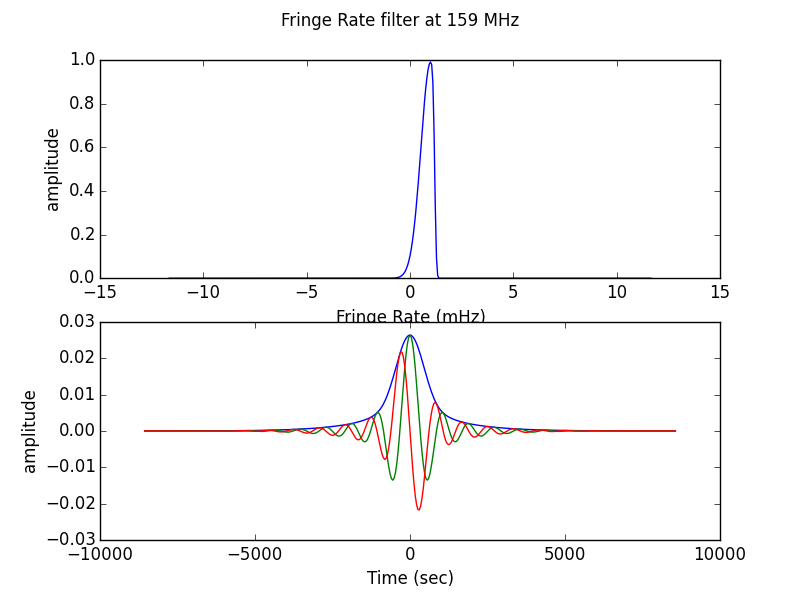
\includegraphics[width=\columnwidth]{plots/fr_filter_slice.png}
\caption{slice of a fringe rate filter at a frequency of 159MHz. Top is the
filter in fringe rate domain. The bottom consists of the corresponding time
domain filter gotten by fourier transforming and windowing with a
blackman-harris window to damp the tails.}
\ref{fig:fringe_rate_cut}
\end{figure}

\begin{figure*}[t!]\centering
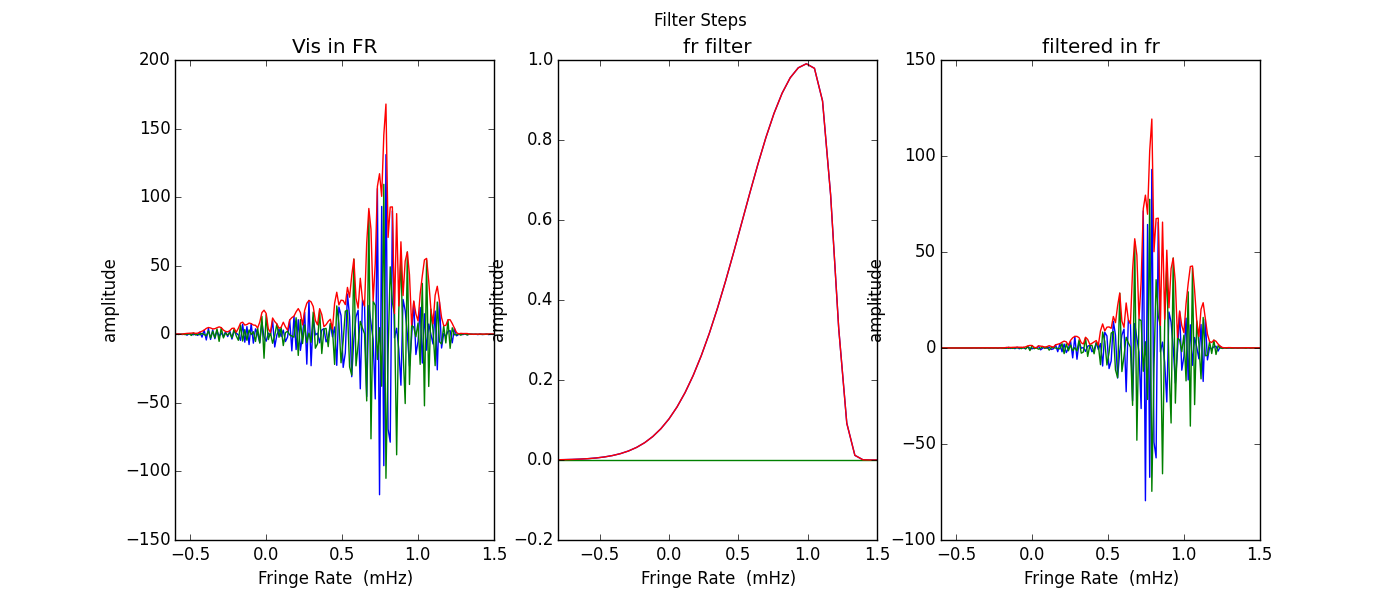
\includegraphics[width=2\columnwidth]{plots/fr_preserved_signal.png}
\caption{slice of a fringe rate filter at a frequency of 159MHz. Shown here is
the fringe-rate transform of foreground contained data for a 30 m east-west
baseline. Blue and green are the real and imaginary part, respectively and red
is the absolute valeu. Note the maximum and minimum fringerates correspond to
the theoretical minimum and maximum for a baseline of this length at 159 MHz.
The center panel shows the real (red)  and imaginary (green) parts of the fringe
rate filter to be applied. Finally, the last panel on the right shows that the
fringe rate filtered visibilities. The fringe rate filter is just a weighting
applied in fringe rate space and retains foregrounds.}
\ref{fig:fr_preserved_signal}
\end{figure*}

\begin{figure}[h!]\centering
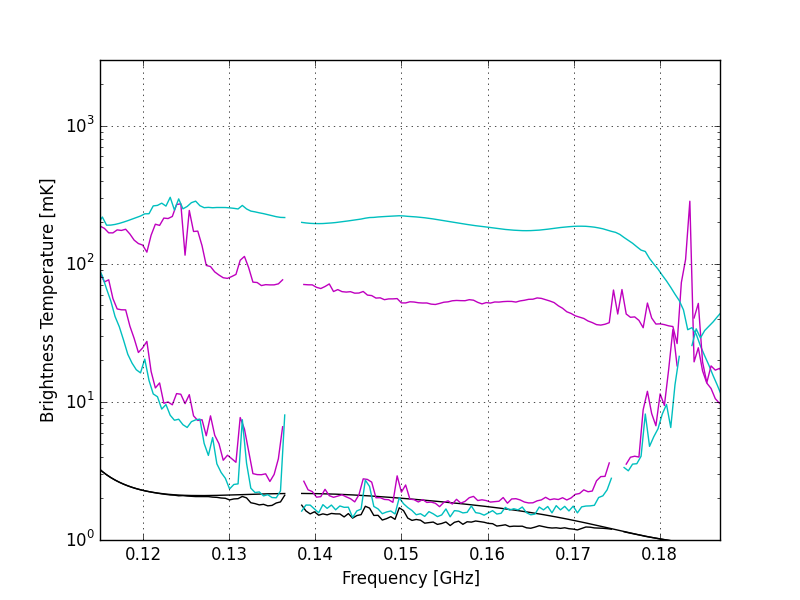
\includegraphics[width=\columnwidth, height=.8\columnwidth]{plots/noise_t.png}
\caption{Estimates of noise temperature. Magenta is frequncy differenced
estimate where the cyan is the time differenced estimate. All curves are
averaged over all 30m east-west baselines (56) and averaged incoherently in 43s
bins of LST from LST 2 to 5 hours with a channel bandwidth of 490 kHz.}
\ref{fig:noise_t}
\end{figure}


%plots:
% filters used. 
% apply filters to foreground data. Compute fr of pica and show that we are not 
%   killing the sky.
% 


\section{Results}

\section{Science}

\section{Conclusions}


%\clearpage
%\nocite{*}
%\bibliographystyle{apj}
%\bibliography{biblio}

\end{document}

